\apendice{Especificación de Requisitos}

\section{Introducción}
En esta sección se trataran los objetivos y requisitos del proyecto. También se definirán los distintos actores que utilizaran la aplicación y se establecerán los  casos de uso de la misma.

\section{Objetivos generales}
Los objetivos generales que se buscan alcanzar  son los siguientes: 
\begin{itemize}
	\item Investigar sobre la comparación de secuencias temporales.
	\item  Investigar distintos métodos de normalización para poder preparar los datos.
	\item Investigar sobre las distintas formas de evaluar la ejecución de ejercicios.
	\item Desarrollar una aplicación con la que el usuario pueda comparar ejercicios de forma sencilla.
\end{itemize}
\section{Catálogo de requisitos}
\subsection{Actores}
Es importante distinguir los roles de los usuarios de la aplicación, a efectos de uso de la misma se pueden distinguir dos roles:
\begin{itemize}
	\item \textbf{Terapeuta}: Persona que se encarga de crear los ejercicios que realizaran los pacientes.
	\item \textbf{Paciente}: Persona que quiere comparar su ejercicio con el del terapeuta.
\end{itemize} 


\subsection{Requisitos funcionales}
En este apartado se trataran los requisitos funcionales de la 
\begin{itemize}
		\item \textbf{RF-1} Gestión de ejercicios
	\begin{itemize}
		\item \textbf{RF-1.1}  El terapeuta podrá crear un ejercicio nuevo.
		\item \textbf{RF-1.2} El terapeuta podrá eliminar un ejercicio existente.
	\end{itemize}
	\item \textbf{RF-2} Selección de ejercicios
	\begin{itemize}
		\item \textbf{RF-2.1}  El terapeuta podrá ver los ejercicios que hay disponibles.
		\item \textbf{RF-2.2} El usuario podrá ver los ejercicios que hay disponibles.
		\item \textbf{RF-2.3} El usuario podrá seleccionar el ejercicio que se va a comparar.
	\end{itemize}
	\item \textbf{RF-3} Gestión de ficheros
	\begin{itemize}
		\item \textbf{RF-3.1}  El terapeuta podrá guardar los ficheros con los datos en la aplicación.
		\item \textbf{RF-3.2} El usuario podrá seleccionar el fichero de datos que se va a comparar.
	\end{itemize}
	\item \textbf{RF-4} Comparación de ejercicios 
	\begin{itemize} 
		\item \textbf{RF-4.1}  El usuario podrá ver una puntuación numérica del ejercicio.
	\end{itemize}
	\item  \textbf{RF-5} Gestión de usuarios
	\begin{itemize}
		\item \textbf{RF-5.1} El usuario  podra crear una cuenta en la aplicación.
		\item \textbf{RF-5.2} El usuario podra iniciar sesión en la aplicación.
		\item \textbf{RF-5.3} El terapeuta podra iniciar sesión en la aplicación.
	\end{itemize}
\end{itemize}
\section{Especificación de requisitos}
En esta sección se especificaran tanto los diagramas de casos de uso como los requisitos necesarios para que la aplicación se pueda desarrollar.
\begin{figure}
	\centering
	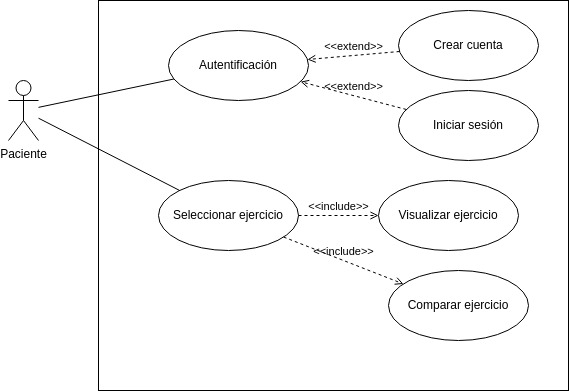
\includegraphics[width=0.7\linewidth]{img/CasosDeUso-Paciente}
	\caption{Diagrama de casos de uso del paciente.}
	\label{fig:casosdeuso-paciente}
\end{figure}

\begin{figure}
	\centering
	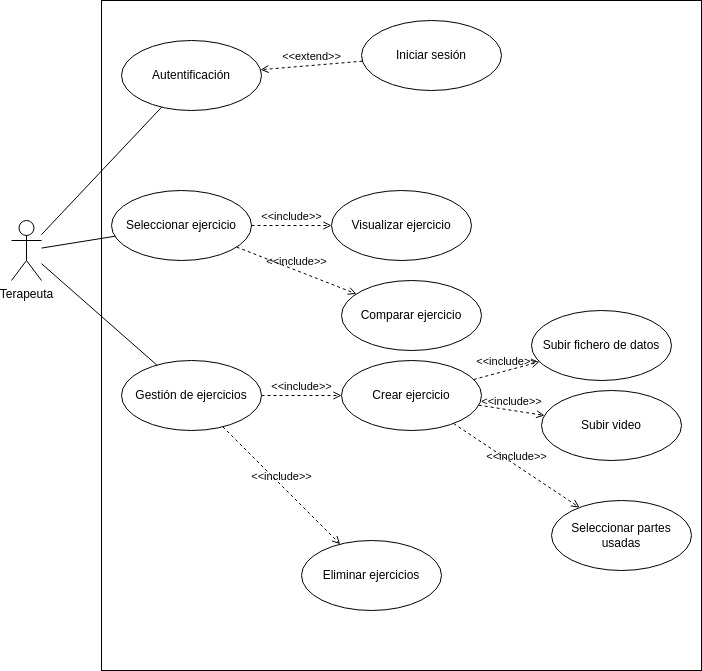
\includegraphics[width=0.7\linewidth]{img/CasosDeUso-Terapeuta}
	\caption{Diagrama de casos de uso del terapeuta.}
	\label{fig:casosdeuso-terapeuta}
\end{figure}


\begin{table}[p]
	\centering
	\begin{tabularx}{\linewidth}{ p{0.21\columnwidth} p{0.71\columnwidth} }
		\toprule
		\textbf{CU-1}    & \textbf{Creación de un nuevo ejercicio}\\
		\toprule
		\textbf{Versión}              & 1.2    \\
		\textbf{Autor}                & Luis Ángel Espinosa Lafuente \\
		\textbf{Requisitos asociados} & RF-1.1 RF-2.1 \\
		\textbf{Descripción}          & Permite al terapeuta crear un ejercicio.  \\
		\textbf{Precondición}         & El terapeuta ha iniciado sesión con una cuenta con el rol correspondiente \\
		\textbf{Acciones}             &
		\begin{enumerate}
			\def\labelenumi{\arabic{enumi}.}
			\tightlist
			\item El terapeuta introduce el nombre del ejercicio.
			\item El terapeuta añade un fichero de datos.
			\item El terapeuta añade un vídeo.
			\item El terapeuta selecciona los ángulos y coordenadas que serán usados para la puntuación.
			\item El terapeuta presiona el botón de confirmar.
		\end{enumerate}\\
		\textbf{Postcondición}        & Ninguna \\
		\textbf{Excepciones}          & Acceso no autorizado en el caso de que el usuario no haya iniciado sesión con el rol de terapeuta  \\
		\textbf{Importancia}          & Alta \\
		\bottomrule
	\end{tabularx}
	\caption{CU-1 Creación de un nuevo ejercicio.}
\end{table}

\begin{table}[p]
	\centering
	\begin{tabularx}{\linewidth}{ p{0.21\columnwidth} p{0.71\columnwidth} }
		\toprule
		\textbf{CU-2}    & \textbf{Eliminación de un ejercicio}\\
		\toprule
		\textbf{Versión}              & 1.1    \\
		\textbf{Autor}                & Luis Ángel Espinosa Lafuente\\
		\textbf{Requisitos asociados} & RF-1.2 RF-2.1 \\
		\textbf{Descripción}          & Permite al terapeuta eliminar un ejercicio.   \\
		\textbf{Precondición}         & 
		\begin{enumerate}		
			\def\labelenumi{\arabic{enumi}.}
			\tightlist
				\item El terapeuta ha iniciado sesión con una cuenta con el rol correspondiente.
				\item El terapeuta ha creado ejercicios previamente. 
		\end{enumerate} \\
		\textbf{Acciones}             &
		\begin{enumerate}
			\def\labelenumi{\arabic{enumi}.}
			\tightlist
			\item El terapeuta selecciona el ejercicio.
			\item El terapeuta presiona el botón de confirmar.
		\end{enumerate}\\
		\textbf{Postcondición}        & Ninguna \\
		\textbf{Excepciones}          & Acceso no autorizado en el caso de que el usuario no haya iniciado sesión con el rol de terapeuta. \\
		\textbf{Importancia}          & Alta \\
		\bottomrule
	\end{tabularx}
	\caption{CU-2 Eliminación de un ejercicio.}
\end{table}

\begin{table}[p]
	\centering
	\begin{tabularx}{\linewidth}{ p{0.21\columnwidth} p{0.71\columnwidth} }
		\toprule
		\textbf{CU-3}    & \textbf{Selección de ejercicio}\\
		\toprule
		\textbf{Versión}              & 1.1    \\
		\textbf{Autor}                &  Luis Ángel Espinosa Lafuente \\
		\textbf{Requisitos asociados} & RF-2.2 RF-2.3 \\
		\textbf{Descripción}          & Permite al usuario ver los ejercicios disponibles y seleccionar el ejercicio que se va a comparar\\
		\textbf{Precondición}         & 
		\begin{enumerate}		
			\def\labelenumi{\arabic{enumi}.}
			\tightlist
			\item El usuario ha iniciado sesión en la aplicación correctamente.
			\item El terapeuta ha creado ejercicios previamente.
		\end{enumerate}\\
		\textbf{Acciones}             &
		\begin{enumerate}
			\def\labelenumi{\arabic{enumi}.}
			\tightlist
			\item El usuario selecciona un ejercicio de un listado.
		\end{enumerate}\\
		\textbf{Postcondición}        & Ninguna \\
		\textbf{Excepciones}          & Acceso no autorizado en el caso de que el usuario no haya iniciado sesión. \\
		\textbf{Importancia}          & Alta \\
		\bottomrule
	\end{tabularx}
	\caption{CU-3 Selección de un nuevo ejercicio.}
\end{table}

\begin{table}[p]
	\centering
	\begin{tabularx}{\linewidth}{ p{0.21\columnwidth} p{0.71\columnwidth} }
		\toprule
		\textbf{CU-4}    & \textbf{Comparación de ejercicio}\\
		\toprule
		\textbf{Versión}              & 1.1    \\
		\textbf{Autor}                &  Luis Ángel Espinosa Lafuente \\
		\textbf{Requisitos asociados} & RF-4.1 \\
		\textbf{Descripción}          & Permite al usuario comparar el ejercicio.\\
		\textbf{Precondición}     &    
		\begin{enumerate}		
			\def\labelenumi{\arabic{enumi}.}
			\tightlist
			\item El usuario ha iniciado sesión en la aplicación.
			\item El usuario ha seleccionado un ejercicio.
			\item El usuario ha seleccionado un fichero.
			\item El fichero se ha cargado correctamente.
		\end{enumerate}\\
		\textbf{Acciones}             &
		\begin{enumerate}
			\def\labelenumi{\arabic{enumi}.}
			\tightlist
			\item El usuario visualiza la puntuación de un ejercicio.
			\item El usuario visualiza el vídeo del ejercicio.
		\end{enumerate}\\
		\textbf{Postcondición}        & Ninguna \\
		\textbf{Excepciones}          & Acceso no autorizado en el caso de que el usuario no haya iniciado sesión \\
		\textbf{Importancia}          & Alta \\
		\bottomrule
	\end{tabularx}
	\caption{CU-4 Comparación de ejercicio.}
\end{table}

\begin{table}[p]
	\centering
	\begin{tabularx}{\linewidth}{ p{0.21\columnwidth} p{0.71\columnwidth} }
		\toprule
		\textbf{CU-5}    & \textbf{Cargar fichero de ejercicio}\\
		\toprule
		\textbf{Versión}              & 1.1    \\
		\textbf{Autor}                &  Luis Ángel Espinosa Lafuente \\
		\textbf{Requisitos asociados} & RF-3.1\\
		\textbf{Descripción}          & Permite al usuario ver los ejercicios disponibles y seleccionar el ejercicio que se va a comparar.\\
		\textbf{Precondición}         & 
		\begin{enumerate}
			\def\labelenumi{\arabic{enumi}.}
			\tightlist
			 \item  El usuario ha iniciado sesión correctamente.
			\item El usuario a seleccionado un ejercicio. 
		\end{enumerate}\\
		\textbf{Acciones}             &
		\begin{enumerate}
			\def\labelenumi{\arabic{enumi}.}
			\tightlist
			\item El usuario selecciona un fichero.
			\item El usuario presiona el botón de confirmar.
		\end{enumerate}\\
		\textbf{Postcondición}        & El usuario ha seleccionado un fichero correctamente. \\
		\textbf{Excepciones}          & Acceso no autorizado en el caso de que el usuario no haya iniciado sesión \\
		\textbf{Importancia}          & Alta \\
		\bottomrule
	\end{tabularx}
	\caption{CU-5 Cargar fichero de ejercicio}
\end{table}


\begin{table}[p]
	\centering
	\begin{tabularx}{\linewidth}{ p{0.21\columnwidth} p{0.71\columnwidth} }
		\toprule
		\textbf{CU-6}    & \textbf{Creación de cuenta}\\
		\toprule
		\textbf{Versión}              & 1.0    \\
		\textbf{Autor}                &  Luis Ángel Espinosa Lafuente \\
		\textbf{Requisitos asociados} & RF-5.1\\
		\textbf{Descripción}          & Permite al usuario crear una cuenta para poder usar la aplicación.\\
		\textbf{Precondición}         & Ninguna\\
		\textbf{Acciones}             &
		\begin{enumerate}
			\def\labelenumi{\arabic{enumi}.}
			\tightlist
			\item El usuario introduce el usuario.
			\item El usuario introduce una contraseña.
			\item El usuario presiona el botón de confirmar.
		\end{enumerate}\\
		\textbf{Postcondición}        & Ninguna \\
		\textbf{Excepciones}          & El usuario ya existe. \\
		\textbf{Importancia}          & Baja \\
		\bottomrule
	\end{tabularx}
	\caption{CU-6 Creación de cuenta.}
\end{table}

\begin{table}[p]
	\centering
	\begin{tabularx}{\linewidth}{ p{0.21\columnwidth} p{0.71\columnwidth} }
		\toprule
		\textbf{CU-7}    & \textbf{Inicio de sesión}\\
		\toprule
		\textbf{Versión}              & 1.0    \\
		\textbf{Autor}                &  Luis Ángel Espinosa Lafuente \\
		\textbf{Requisitos asociados} & RF-5.2 RF-5.3\\
		\textbf{Descripción}          & El usuario podrá iniciar sesión para poder acceder a la aplicación.\\
		\textbf{Precondición}         & El usuario tiene una cuenta.\\
		\textbf{Acciones}             &
		\begin{enumerate}
			\def\labelenumi{\arabic{enumi}.}
			\tightlist
			\item El usuario introduce el usuario.
			\item El usuario introduce una contraseña.
			\item El usuario presiona el botón de confirmar.
		\end{enumerate}\\
		\textbf{Postcondición}        & Ninguna \\
		\textbf{Excepciones}          & Usuario o contraseña incorrectos. \\
		\textbf{Importancia}          & Baja \\
		\bottomrule
	\end{tabularx}
	\caption{CU-7 Inicio de sesión.}
\end{table}

